%!TEX root = ../main.tex

\chapter{State of the Art}
\label{chp:stateOfArt}

Geometrical representations of words are the building blocks in the field of \ac{NLP}, for higher-level tasks such as word sense disambiguation, sentiment analysis, and language modeling. The efforts for developing static word embeddings go all the way back to the 1980s, and currently there are many models in the literature each approaching the problem with a different methodology.

In this chapter, we will list and briefly describe some of the most known static word embedding models. This background will be later useful to demonstrate how our approach differs from others.

\section{word2vec}

One work that established a fundamental step in the field of \ac{NLP} is word2vec, which was presented in the article \cite{w2v} by Tomas Mikolov, Kai Chen, Greg Corrado, and Jeffrey Dean. More precisely, in this article, the authors present a shallow neural network-based training of two different architectures, namely, \ac{CBOW} and \ac{SG}.

For each word in the vocabulary, word2vec produces a vector, which is typically of several hundred dimensions. The training procedure organizes the vector space in such a way that if two words share similar contexts, i.e. they are both surrounded by the same words, then the two vectors associated with them are close to each other. Consequently, similar words like “car” or “automobile”, or related terms, like “fork” and “spoon”, will have similar vectors, considering that they have similar contexts in the training corpus. 

\begin{figure}[h]
    \centering
    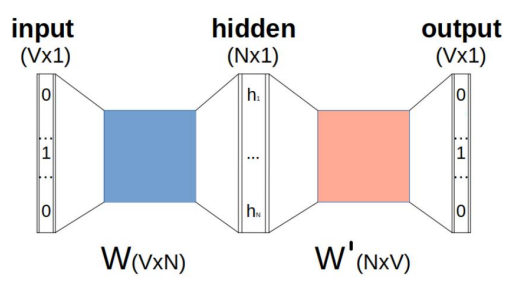
\includegraphics[width=0.8\textwidth]{img/g1.PNG}
    \caption{Generic word2vec architecture}
    \label{fig:g1}
\end{figure}

word2vec models are trained via an unsupervised approach, by feeding the neural network a large corpus with unannotated types in it. The network is trained with gradient descent to perform a particular task different from the one of interest. There is no activation function on the hidden neurons layer, and the output neurons use the softmax function. After training, the output layer is discarded, keeping only the input layer, which represents the target of interest. In this specific case, the network is trained to optimize an objective function to answer the question "Is the word $w$ likely to appear near the word $c$?". Subsequently, the input layer parameters will constitute the searched word embeddings.

\subsection{CBOW}

\ac{CBOW} model aims to train a neural network in such a way that it can predict a central word, given a fixed window of $2L$ words in its context. That is, if the system input is a text of a given length, consider $w_t$ the current central word (in the example “pepper”) and $w_i$ with $i = t - L, t - L + 1, ..., t + L - 1, t + L$ the words in its context, i.e. the words close to it in the corpus (in the example if $L = 2$, the context words are “cinnamon”, “salt”, “allspice” and “pine”), then the purpose of the model is to predict $w_t$ given $w_i$.

\begin{table}[!h]
\centering
\begin{tabular}{cccccccc}
seasoned & with & cinnamon, & salt, & pepper, & allspice, & pine & nuts \\
$w_{t-4}$ & $w_{t-3}$ & $w_{t-2}$ & $w_{t-1}$ & $w_{t}$ & $w_{t-+1}$ & $w_{t+2}$ & $w_{t+3}$
\end{tabular}
\end{table}

%To do this, the network is constructed as in Figure 3.2.

%\begin{figure}[h]
%    \centering
%    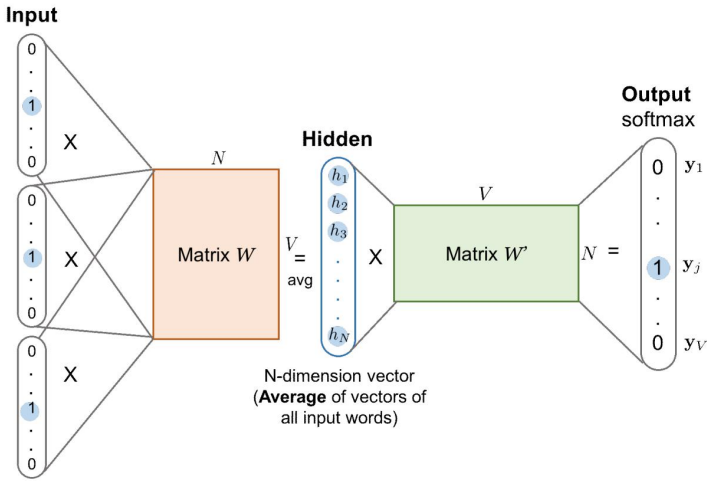
\includegraphics[width=0.95\textwidth]{img/g2.PNG}
%    \caption{CBOW architecture}
%    \label{fig:g2}
%\end{figure}

%This network has as input the 2L one-hot representations of the context words wi , each of 
The network constructed for this task has as input the $2L$ one-hot representations of the context words $w_i$, each of size $|V| \times 1$, with $|V|$ the size of the vocabulary. The hidden layer is composed of a vector $h$ of size $N \times 1$, with $N$ being the dimension of the word embeddings. The value of the hidden layer is calculated as the average of the vectors corresponding to the input context words transformed by the input weights matrix $W$., i.e.

\[
h = \frac{1}{2L}\sum_{i=-L, i \neq 0}^{L} x_{t-1}^{T} W_{(N \times |V|)}
\]

Subsequently, the product $W'h$ is calculated, where $W'$ is the matrix of hidden weights, obtaining a vector $z$ of dimension $|V| \times 1$. The output is then calculated from $z$ via the softmax function so that the output layer reports for each word $y_i$ in the vocabulary, the probability that it is the central term considering the context given in input. Finally, assuming that the node with the highest probability is $y_s$, the output one-hot vector will be the one with value $1$ in the $s$-th component and with all the remaining components set to 0.

%This model has as parameters two weight matrices W and Wÿ such that:

%\begin{itemize}
%    \item  W ÿ RN×|V | it is the matrix that will contain the embeddings of the words considered as central words
%    \item  Wÿ ÿ R|V |×N is the matrix that will contain the embeddings of the words considered as context words.
%\end{itemize}

Once the training is complete, the rows of matrix $W$ will be the desired word embeddings, corresponding to each word in the vocabulary.


\subsection{Skip-Gram}

Now we focus on how the Skip-Gram model works. Starting from a word in the middle of a sentence, called the \textit{central word}, consider the words surrounding it within a $2L$-sized window, called \textit{context words}. Differently from \ac{CBOW}, this model aims to predict the context words starting from the central word through the optimization of an objective function. The model scheme is represented in Figure \ref{fig:g3}.

\begin{figure}[h]
    \centering
    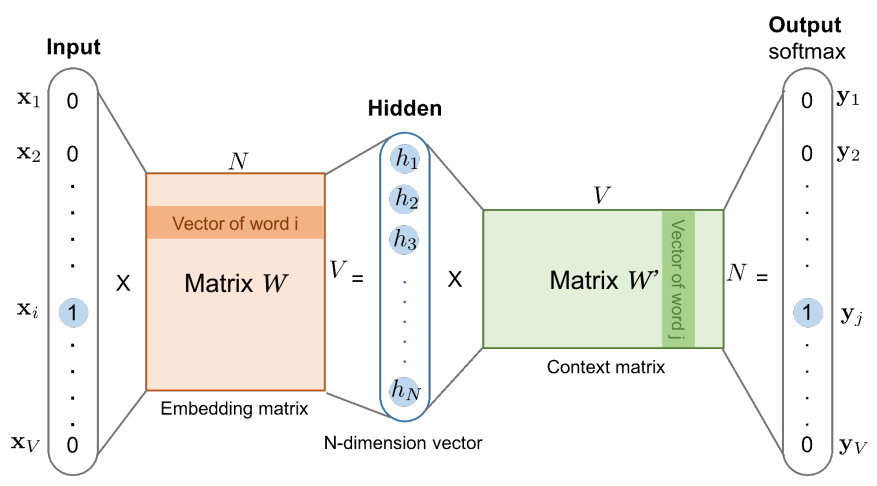
\includegraphics[width=0.95\textwidth]{img/g3.PNG}
    \caption{Skip-Gram architecture}
    \label{fig:g3}
\end{figure}

We see that the model input is a one-hot vector $x$, of dimension $|V| \times 1$, pointing to the current central word $w_t$. The output of the network consists of a single vector containing a probability distribution on all the vocabulary items, where each component represents how probable it is to find the corresponding vocabulary word in the vicinity of the central word.

%An important assumption is that given a central word, the various context words are completely independent %and identically distributed between them (iid). In other words, all the words within the considered window %are treated in the same way with respect to the input word, i.e. different sets of probabilities are not %learned based on the distance from the input.

Similarly to \ac{CBOW} the parameters are organized into two matrices $W$ and $W'$, which connect the input layer to the hidden layer, and the hidden layer to the output layer, respectively.

\begin{itemize}
    \item $W \in R^{N \times |V|}$ is the matrix of embeddings of the \textbf{input} words: the $i$-th row corresponds to the embedding of the word $w_i$ when it is considered as a central word. We denote this vector with $v_{w_i}$. It is also called the \textit{target embedding} of the word $w_i$.
    \item $W' \in R^{N \times |V|}$ is the matrix of embeddings of the \textbf{output} words: the $i$-th row corresponds to the embedding of the word $w_i$ when it is considered as a context word. We denote this vector with $u_{w_i}$. It is also called the \textit{context embedding} of the word $w_i$.
\end{itemize}

In the hidden layer, which has $N$ nodes matching with the dimensionality of the word embeddings, obtained with the product of the one-hot vector $x$ relating to the central word $w_I$ and the weight matrix $W$, as:

\[
h = x^T W = v_{w_{I}}
\]
\noindent
i.e. the word embedding of the input word, when this is seen as the central word (vector of the $I$-th row of $W$).

The output layer can be seen as a softmax regression classifier where each output neuron produces a value between 0 and 1, and all these output values sum to 1. Indeed, by multiplying $W'h$, we obtain a vector $z$ of size $|V| \times 1$, in which each component will be proportional to the similarity of $h$ and the embedding of the $i$-th word of the dictionary represented in $W'$. Specifically, each weight vector belongs to the matrix $W'$ multiplied with the vector obtained from the hidden layer, where $u$ is calculated.

The softmax function is then applied to the result:

\begin{equation}
\label{math:wo-wi}
p(w_O|w_I) = \text{softmax}(u_{w_O}^T v_{w_I}) = \frac{exp(u_{w_O}^T v_{w_I})}{\sum_{w=1}^{V} exp(u_w^T v_{w_I})}
\end{equation}
\noindent
obtaining the probability of predicting a context word $w_O$ given $w_I$.

Given a sequence of training words $w_1, ..., w_T$, let $L$ be the size of the window, the objective function to be maximized can be formalized as follows:

\[
\frac{1}{T}\sum_{t=1}^T \sum_{-L \leq j \leq L, j \neq 0} \log{P(w_{t+j} | w_t)}
\]
\noindent
where the probabilities $P(w_{t+j} | w_t)$ can be calculated as in Formula \ref{math:wo-wi}.

\subsubsection{Skip-Gram with Negative Sampling}

\ac{SGNS} is Skip-Gram combined with the strategy that is a simplified variation of \ac{NCE}, which was introduced in \cite{nce}. \ac{NCE} is based on the idea of using a logistic regression classifier to distinguish data from noise. \textit{Negative sampling}, on the other hand, can be considered a simplification of it and it focuses on learning the contrastive relationship of words, rather than just learning embeddings to position similar words close to each other.

The basic steps of \ac{SGNS} are:

\begin{itemize}
    \item Select each pair of central word and context words from the $L$-size window surrounding the central word, as \textit{positive examples}.
    \item Select by following some probability distribution the words from the vocabulary to pair with the central word to create the \textit{negative examples}.
    \item Use logistic regression to train a classifier that distinguishes positive examples from negative ones.
    \item The weights learned through logistic regression are the desired embeddings.
\end{itemize}

Given a pair of words $(w, c)$ with $w$ the central word and $c$ the candidate word in its context, we define with $P(+|w, c)$ the probability that $c$ is a word in the real context of $w$. The probability that $c$ is not a word in the context of w is defined as $P(-|w, c) = 1 - P(+|w, c)$. The calculation of these probabilities is based on the intuition that two words co-occur if their embeddings are similar. Embeddings are said to be similar if their scalar product is high. Therefore the concept of similarity between two embeddings was defined as $\mathit{sim}(w, c) = c \cdot w$. To transform this scalar product into a probability, the Sigmoid function ($\sigma$) is used. The definition of the Sigmoid function is presented in Section \ref{sec:sigmoid}.

Therefore the probability that a word $c$ is not in the context of $w$ is:

\[
P(-|w,c) = 1 - P(+|w,c) = \sigma(-c \cdot w) = \frac{1}{1+ \exp (c \cdot w)}
\]
\noindent 
so that the total probability of the two events “\textit{$c$ is in context}” and “\textit{$c$ is not in context}” add to one. These equations define the probability for a single pair of a central word and a context word, however, the model does not consider a single context word for each central word but a set of context words within a window.

With the assumption in the word2vec model, that is, for given a central word, the various context words are completely independent and identically distributed, to obtain the probability that a set of $c_{-L:L}$ words is in the context of another, it is possible to multiply the probabilities associated with each pair:

\[
P(+|w,c_{-L:L}) = \prod _ {i=-L, i \neq 0} ^L \sigma(c_i \cdot w)
\]

\[
P(+|w,c_{-L:L}) = \prod _ {i=-L, i \neq 0} ^L \log \sigma(c_i \cdot w)
\]

The purpose of this model is, therefore, to maximize the similarity between the words belonging to the pairs of positive examples, and minimize the similarity of pairs belonging to the negative examples.

If we consider a word-context pair $(w, c_\mathit{pos})$ and $k$ noise words $c_{\mathit{neg}_1}, ..., c_{\mathit{neg}_k}$, we can express these two objectives with the following single loss function:

\begin{align}
LOSS &= - \log(P(+|w, c_\mathit{pos}) \prod_{i=1}^k P(- | w, c_{\mathit{neg}_i}))  \\
&= -(\log P(+|w, c_\mathit{pos}) + \sum_{i=1}^k \log P(-|w,c_{\mathit{neg}_i})) \\
&= -(\log P(+|w, c_\mathit{pos}) + \sum_{i=1}^k \log (1 - P(+|w, c_{\mathit{neg}_i}))) \\
&= - (\log \sigma(c_\mathit{pos} \cdot w) + \sum_{i=1}^{k} \log \sigma(-c_{\mathit{neg}_i} \cdot w))
\end{align}

where the first term expresses the fact that we want the classifier to assign the real context word $c_\mathit{pos}$ a high probability of being close, and the second term expresses the fact that we want to assign each of the noise words $c_{\mathit{neg}_i}$ a high probability of being a non-neighbor. These two terms must be multiplied, again due to the fact that independence has been assumed between the context words, and therefore between the pairs of examples.

\newpage

\section{GloVe}

\ac{GloVe}, presented in \cite{glove}, is an unsupervised learning algorithm to obtain good-quality vector representations for words. It has the benefits of both methods based on matrices of global co-occurrence statistics, which are particularly effective in capturing the similarity between words, and effective models based on \ac{DL} techniques, such as word2vec in grasping analogies and complex structures. The advantage of \ac{GloVe} is that, unlike word2vec, is not based only on local statistics (contextual information local of words), but also incorporates global statistics (co-occurrence of words) to get word vectors. 

GloVe is based on an important idea,

\begin{displayquote}
\centering
"You can derive semantic relationships between words from the co-occurrence matrix."
\end{displayquote}

Given a corpus of V words, the co-occurrence matrix $X$ will be a matrix $|V| \times |V|$, where the element $X_{ij}$, corresponding to the $i$-th row and $j$-th column of $X$, indicates how many times does the word $i$ appear close to the word $j$.

%\begin{table}[h]
%\centering
%\begin{tabular}{cccccc}
% & \textbf{the} & \textbf{cat} & \textbf{sat} & \textbf{on} & \textbf{mat} \\
%\textbf{the} & 0 & 1 & 0 & 1 & 1 \\
%\textbf{cat} & 1 & 0 & 1 & 0 & 0 \\
%\textbf{sat} & 0 & 1 & 0 & 1 & 0 \\
%\textbf{on} & 1 & 0 & 1 & 0 & 0 \\
%\textbf{mat} & 1 & 0 & 0 & 0 & 0
%\end{tabular}
%\caption{Co-occurrence matrix}
%\label{tab:g2}
%\end{table}

Let $P_{ik} = \frac{X_{ik}}{X_i}$ the probability of seeing the word $i$ and $k$ together, calculated by dividing the number of times $i$ and $k$ appear together, by times the total number of times in which $i$ appeared in the corpus. For example, consider Table \ref{tab:g3}.
%in which the probabilities that the target words ice are represented and steam co-occur with various probe words k from the vocabulary:

\begin{itemize}
    \item  if $k$ is very similar to \textit{ice} but irrelevant for \textit{steam} (e.g. $k$ = \textit{solid}),  $\frac{P_{ik}}{P_{jk}}$, very high ($>1$)
    \item if $k$ is very similar to \textit{steam} but irrelevant to \textit{ice} (e.g. $k$ = \textit{gas}), small ($<1$), $\frac{P_{ik}}{P_{jk}}$ will be high
    \item if k is related or unrelated to any of the words (e.g. $k$ = \textit{fashion}), $\frac{P_{ik}}{P_{jk}}$ will be close to 1
\end{itemize}


\begin{table}[h]
\centering
\begin{tabular}{|c|cccc|}
\hline
probability and ratio & \textbf{k=solid} & \textbf{k=gas} & \textbf{k=water} & \textbf{k=fashion} \\ \hline
\textbf{P(k|ice)} & $1.9 \times 10^{-4}$ & $6.6 \times 10^{-5}$ & $3 \times 10^{-3}$ & $1.7 \times 10^{-5}$ \\
\textbf{P(k|steam)} & $2.2 \times 10^{-5}$ & $7.8 \times 10^{-4}$ & $2.2 \times 10^{-3}$ & $1.8 \times 10^{-5}$ \\
\textbf{P(k|ice)/P(k|steam)} & $8.9$ & $8.5 \times 10^{-2}$ & $1.36$ & $0.96$ \\ \hline
\end{tabular}
\caption{$P_{ik}/P_{jk}$ behavior}
\label{tab:g3}
\end{table}

%Consider how the authors reasoned when designing this model: first of all they posed three problems, then they found the solutions and created the model.

%\begin{enumerate}
%    \item $\frac{P_{ik}}{P_{jk}}$ is not an equation, but just an expression.
%    \item Word vectors are high-dimensional vectors, however, Pik So there is a $\frac{P_{ik}}{P_{jk}}$ it is a scalar. Therefore there is a dimensional mismatch.
%    \item  There are three entities involved (i, j and k) but the authors want to reduce the function of loss to the calculation with only two entities.
%\end{enumerate}

The authors considered two different levels of word embeddings, $u$ and $w$, to reduce overfitting. They assumed that there exists a function $F$ that accepts the vectors associated with the words $i$, $j$ and $k$, and returns the ratio of interest:
%To answer problem 1, they assumed that there exists a function F that accepts the vectors associated with the words i, j and returns the ratio of interest:

\[
F(w_i, w_j, u_k) = \frac{P_{ik}}{P_{jk}}
\]

Then, they observed how the distance between two different words $i$ and $k$, calculated with respect to the vector $w_i - w_j$, is related to the reciprocal of $P_{ik}$ (Figure \ref{fig:g6}).

So they thought of changing the above equation to the following:

\[
F(w_i - w_j, u_k) = \frac{P_{ik}}{P_{jk}}
\]

\begin{figure}[h]
    \centering
    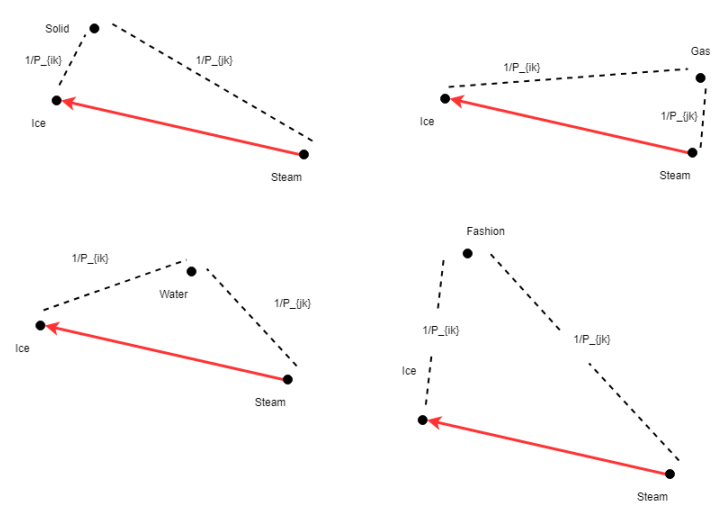
\includegraphics[width=0.95\textwidth]{img/g6.PNG}
    \caption{Behavior of vector distances with respect to $w_i - w_j$}
    \label{fig:g6}
\end{figure}

Then the authors introduced a transposition and a dot product as follows:
%To solve problem 2, the authors introduced a transposition and a dot product as follows:

\[
F((w_i - w_j)^\top u_k) = \frac{P_{ik}}{P_{jk}}
\]

They assumed that $F$ had an important property: homomorphism, so that they could write:

\[
F(w_i^\top u_k - w_j^\top u_k) = \frac{F(w_i^\top u_k)}{F(w_j^\top u_k)} = \frac{P_{ik}}{P_{jk}}
\]
\noindent
In other words, this homomorphism means that the subtraction $F(A-B)$ can be represented as a division $F(A)/F(B)$ and the two operations obtain the same result. And therefore,

\[
\frac{F(w_i^\top u_k)}{F(w_j^\top u_k)} = \frac{P_{ik}}{P_{jk}}
\]
\noindent
and, 

\[
F(w_i^\top u_k) = P_{ik}
\]
\noindent
The above relationship should be defined as:

\[
F(w_i^\top u_k) = c P_{ik}
\]
\noindent
for some constant $c$, considering that we cannot always assume that, given \\$F(A)/F(B) = G(A)/G(B)$, $F(A) = G(A)$ holds or that, given \\$F(A)/F(B) = 2F(A)/2F(B)$, $F(A) = 2F(A)$ holds. However in this case, if the similarity between $i$ and $k$ increases by a constant $c$, the similarity between $j$ and $k$ (for any $j$) will also increase by $c$. This means that all word vectors would be scaled by a factor $c$, which does not create a real problem and therefore the above can be assumed.

They set $F$ equal to the exponential function to enforce the property of homomorphism mentioned above: 

\[
\exp(w_i^\top u_k) = P_{ik} = \frac{X_{ik}}{X_i}
\]
\noindent
and therefore:

\[
w_i^\top u_k = \log X_{ik} - \log X_{i}
\]
\noindent
Since $X_i$ is independent of $k$ we can move it to the left:

\[
w_i^\top u_k + \log X_{i}= \log X_{ik}
\]
\noindent
Then they added some bias into the equation, we express $\log X_{i}$ as

\[
w_i^T u_k + bw_i + bu_k = \log(X_{ik}) 
\]
\[
w_i^T u_k + bw_i + bu_k - \log(X_{ik}) = 0
\]
\noindent
where $b_w$ and $b_u$ are network bias.

They observed that in an ideal environment, where you have perfect word vectors, the above expression would equal zero. Then they set the model's objective to minimize the following cost function:

\[
J(w_i, w_j) = (w_i^\top u_j + bw_i + bu_j - \log(X_{ij}))^2
\]

Then we come across a problem when $X_{ik} = 0$, which is the state when our cost function yields $\mathit{NaN}$, given that $log(0)$ is undefined. The GloVe authors proposed a smart solution: introducing a function $f(X_{ij})$ which weights words based on their frequency, in which infrequent words will have smaller weights. The \ac{GloVe} loss function is then:

\[
J = f(X_{ij})(w_i^\top u_j + bw_i + bu_j - \log(X_{ij}))^2
\]
\noindent
where $f(X_{ij})$ is defined as:

\[
f(X_{ij}) = 
\begin{cases}
(x/x_{\max})^a & \text{ if } x < x_{\max}\\ 
0 & \text{ otherwise}
\end{cases}.
\]

%Note that obtaining the co-occurrence matrix requires a single pass through the entire corpus to collect the required statistics. For a large corpus, this step can be computationally expensive, but it is a one-time cost upfront.

%\newpage


%\section{fastText}

%FastText is an extension of the word2vec architecture released by Facebook AI Research in 2016 [5]. FastText is %also an open-source library that allows users to learn text representations and text classifiers, available in %several languages.

%Instead of directly learning vectors for individual words, fastText represents each word as 
%an n-gram of characters. So, for example, if you take the word “artificial” with n = 3, the 
%fastText representation of this word is “ar, art, rti, tif, ifi, fic, ici, ial, al”. Once each word has 
%been represented using n-grams, we proceed as in word2vec: the neural network of the 
%word2vec model is trained to learn the embeddings and those of the corresponding matrix 
%are taken as word embeddings. Proceeding in this way, the authors highlighted how this 
%method allows embeddings to include suffixes and prefixes.


%FastText works well with rare words, without considering morphological inflection or other 
%lexical derivations (prefix or suffix): simply put, FastText aims to predict a category rather 
%than a word. Furthermore, this architecture features a hierarchical softmax.

%An important advantage of this method is that it can create word embeddings even for 
%words not seen in the training corpus. Indeed, if a word was not seen during training, it can 
%still be split into n-grams to obtain its embeddings. Both word2vec and GloVe, however, 
%do not provide any vector representation for words that are not in the dictionary of the model.
